\chapter{Kombinatoriikka}
% 
% Kombinatoriikka tarkoittaa yhdistelmien määrän laskemista.
% Tavoitteena on yleensä laskea yhdistelmät
% tehokkaasti niin, että jokaista yhdistelmää
% ei tarvitse muodostaa erikseen, vaan yhteismäärän
% saa selville tehokkaammin hyödyntämällä säännöllisyyksiä ja
% dynaamista ohjelmointia.

\section{Perustekniikat}

\section{Binomikerroin}

Binomikerroin ${n \choose k}$ ilmaisee, montako
$k$ alkion osajoukkoa $n$ alkion joukosta
voidaan muodostaa.
Esimerkiksi ${5 \choose 2}=10$,
koska 5 alkion joukosta $\{A,B,C,D,E\}$
voidaan muodostaa seuraavat 10 osajoukkoa, joissa on 2 alkiota:
\[ \{A,B\}, \{A,C\}, \{A,D\}, \{A,E\}, \{B,C\}, 
\{B,D\}, \{B,E\}, \{C,D\}, \{C,E\}, \{D,E\} \]

\subsubsection{Laskutapa 1}

Binomikertoimen voi laskea rekursiivisesti seuraavasti:

\[
{n \choose k}  =  {n-1 \choose k-1} + {n-1 \choose k}
\]

Ideana rekursiossa on tarkastella tiettyä
joukon alkiota $x$.
Jos alkio $x$ valitaan osajoukkoon,
täytyy vielä valita $n-1$ alkiosta $k-1$ alkiota.
Jos taas alkiota $x$ ei valita,
täytyy vielä valita $n-1$ alkiosta $k$ alkiota.

Rekursion pohjatapaukset ovat seuraavat:

\[
{n \choose 0}  =  {n \choose n} = 1
\]

Selityksenä on, että tyhjän osajoukon voi muodostaa
aina yhdellä tavalla, samoin kuin osajoukon,
jossa on kaikki joukon alkiot.

\subsubsection{Laskutapa 2}

Toinen tapa laskea binomikerroin on seuraava:
\[
{n \choose k}  =  \frac{n!}{k!(n-k)!}.
\]
Kaavassa $n!$ on $n$ alkion joukon permutaatioiden määrä.
Ideana on käydä läpi joukon permutaatiot
ja valita kussakin tapauksessa
permutaation $k$ ensimmäistä lukua osajoukkoon.
Koska lukujen järjestyksellä osajoukossa
ja osajoukon ulkopuolella ei ole väliä,
tulos jaetaan luvuilla $k!$ ja $(n-k)!$.

\subsubsection{Ominaisuuksia}

Binomikertoimelle pätee
\[
{n \choose k}  =  {n \choose n-k},
\]
koska $k$ alkion valinta $n$ alkiosta
tarkoittaa samaa kuin että valitaan
$n-k$ alkiota, joita ei oteta mukaan.

Binomikerrointen summa on
\[
{n \choose 0}+{n \choose 1}+{n \choose 2}+\ldots+{n \choose n}=2^n.
\]

Nimi ''binomikerroin'' tulee siitä, että

\[ (a+b)^n =
{n \choose 0} a^n b^0 + 
{n \choose 1} a^{n-1} b^1 +
\ldots + 
{n \choose n-1} a^1 b^{n-1} +
{n \choose n} a^0 b^n. \]
Binomikertoimet esiintyvät myös Pascalin
kolmiossa, jonka reunoilla on lukua 1
ja jokainen luku saadaan
kahden yllä olevan luvun summana:
\begin{center}
\begin{tikzpicture}{0.9}
\node at (0,0) {1};
\node at (-0.5,-0.5) {1};
\node at (0.5,-0.5) {1};
\node at (-1,-1) {1};
\node at (0,-1) {2};
\node at (1,-1) {1};
\node at (-1.5,-1.5) {1};
\node at (-0.5,-1.5) {3};
\node at (0.5,-1.5) {3};
\node at (1.5,-1.5) {1};
\node at (-2,-2) {1};
\node at (-1,-2) {4};
\node at (0,-2) {6};
\node at (1,-2) {4};
\node at (2,-2) {1};
\end{tikzpicture}
\end{center}

\subsubsection{Laatikot ja pallot}

Laatikot ja pallot on usein hyödyllinen malli
kombinatoriikan tehtävissä.
Siinä $n$ laatikkoon sijoitetaan $k$ palloa.
Tarkastellaan seuraavaksi kolmea tapausta:

\textit{Tapaus 1}: Kuhunkin laatikkoon saa sijoittaa
enintään yhden pallon.
Sijoitustapojen määrä on ${n \choose k}$.

\textit{Tapaus 2}: Samaan laatikkoon saa sijoittaa
monta palloa.
Sijoitustapojen määrä on ${n+k-1 \choose k}$.

Prosessin voi kuvata merkkijonona, joka muodostuu
merkeistä ''o'' ja ''$\rightarrow$''.
Pallojen sijoittaminen alkaa
vasemmanpuoleisimmasta laatikosta.
Merkki ''o'' tarkoittaa, että pallo sijoitetaan
nykyiseen laatikkoon, ja merkki
''$\rightarrow$'' tarkoittaa, että siirrytään
seuraavaan laatikkoon.

Nyt jokainen sijoitustapa on merkkijono, jossa
on $k$ kertaa merkki ''o'' ja $n-1$ kertaa
merkki ''$\rightarrow$''.
Niinpä sijoitustapojen määrä on ${n+k-1 \choose k}$.

\textit{Tapaus 3}: Kuhunkin laatikkoon saa sijoittaa
enintään yhden pallon ja lisäksi missään kahdessa
vierekkäisessä laatikossa ei saa olla palloa.
Sijoitustapojen määrä on ${n-k+1 \choose n-2k+1}$.

Tässä tapauksessa voi ajatella, että $k$ palloa
ovat laatikoissaan ja joka välissä on ainakin
yksi tyhjä laatikko.
Niinpä jää valittavaksi $n-k-(k-1)=n-2k+1$ laatikon paikat.
Mahdollisia välejä on $k+1$, joten tapauksen 2 perusteella
sijoitustapoja on ${k+1+n-2k+1-1 \choose n-2k+1} = {n-k+1 \choose n-2k+1}$.

\subsubsection{Multinomikerroin}

Binomikertoimen yleistys on multinomikerroin

\[ {n \choose k_1,k_2,\ldots,k_m} = \frac{n!}{k_1! k_2! \cdots k_m!}, \]

missä $k_1+k_2+\cdots+k_m=n$.
Multinomikerroin ilmaisee, monellako tavalla $n$ alkiota voidaan jakaa osajoukkoihin,
joiden koot ovat $k_1,k_2,\ldots,k_m$.
Jos $m=2$, multinomikertoimen kaava vastaa binomikertoimen kaavaa.

\section{Catalanin luvut}

Catalanin luku $C_n$ ilmaisee,
montako tapaa on muodostaa kelvollinen sulkulauseke
$n$ alkusulusta ja $n$ loppusulusta.
Esimerkiksi $C_3=5$, koska 3 alkusulusta
ja 3 loppusulusta voidaan muodostaa
kelvolliset sulkulausekkeet
\texttt{()()()}, \texttt{(())()},
\texttt{()(())}, \texttt{((()))} ja \texttt{(()())}.

\subsubsection{Sulkulausekkeet}

Sulkulauseke on kelvollinen, jos sen pystyy
muodostamaan jostakin
matemaattisesta lausekkeesta poistamalla
kaikki merkit sulkuja lukuun ottamatta.
Esimerkiksi sulkulauseke \texttt{(())()}
on kelvollinen, koska sitä vastaa
matemaattinen lauseke $(2 \cdot (4+5)+3)\cdot(1+3)$.

Kelvollisen sulkulausekkeen voi tunnistaa käymällä
läpi lausekkeen merkit vasemmalta oikealle ja
pitämällä yllä laskuria, jonka arvo on aluksi 0.
Merkki \texttt{(} kasvattaa laskuria ja
merkki \texttt{)} vähentää laskuria.
Sulkulauseke on kelvollinen, jos laskurin arvo
on aina vähintään 0 ja lopuksi tasan 0.

Huomaa myös, että kelvollisen sulkulausekkeen
jokaisessa alkuosassa alkusulkujen määrä on
sama tai suurempi kuin loppusulkujen määrä.

\subsubsection{Laskutapa 1}

Catalanin lukuja voi laskea rekursiivisesti seuraavasti:
\[ C_n = \sum_{i=1}^{n} C_{i-1} C_{n-i}\]
Ideana on käydä läpi vaihtoehdot
jakaa sulkulauseke kahteen osaan niin,
että kumpikin osa on kelvollinen sulkulauseke
ja alkuosa on mahdollisimman lyhyt mutta ei tyhjä.
Muuttuja $i$ ilmaisee, montako sulkuparia
alkuosassa on.
Kunkin vaihtoehdon kohdalla lausekkeiden määrä
saadaan kertomalla keskenään:

\begin{itemize}
\item $C_{i-1}$: tavat muodostaa sulkulauseke
alkuosan sulkupareista ulointa sulkuparia lukuun ottamatta
\item $C_{n-i}$: tavat muodostaa sulkulauseke
loppuosan sulkupareista
\end{itemize}
Lisäksi pohjatapauksena on $C_0=1$, koska 0
sulkuparista voi muodostaa
tyhjän sulkulausekkeen.

\subsubsection{Laskutapa 2}

Catalanin lukuja voi laskea myös binomikertoimen avulla:
\[ C_n = \frac{1}{n+1} {2n \choose n}. \]
Kaavan voi perustella laskemalla, moniko $n$ alkusulkua
ja $n$ loppusulkua sisältävä sulkulauseke \textit{ei}
ole kelvollinen.
Sulkulausekkeita on kaikkiaan ${2n \choose n}$,
koska lausekkeessa on $2n$ merkkiä ja siitä valitaan
$n$ kohtaa alkusuluille.

Jos sulkulauseke ei ole kelvollinen,
siinä on alkuosa, jossa loppusulkuja on alkusulkuja
enemmän.
Ideana on kääntää jokainen tällaisen alkuosan
sulkumerkki.
Esimerkiksi lausekkeessa \texttt{())()(}
alkuosa on \texttt{())}, joten kääntämisen
jälkeen lausekkeesta tulee \texttt{)((()(}.

Tuloksena olevassa lausekkeessa on $n+1$ alkusulkua
ja $n-1$ loppusulkua. Tällaisia lausekkeita on
kaikkiaan ${2n \choose n+1}$, joten kelvollisten
sulkulausekkeiden määrä voidaan laskea kaavalla
\[{2n \choose n}-{2n \choose n+1} = {2n \choose n} - \frac{n}{n+1} {2n \choose n} = \frac{1}{n+1} {2n \choose n}.\]

\subsubsection{Binääripuut}

Toinen tulkinta Catalanin luvuille on,
että $C_n$ on $n$ alkion binääripuiden määrä.
Esimerkiksi $C_3=5$ ja vastaavat binääripuut ovat:

\begin{center}
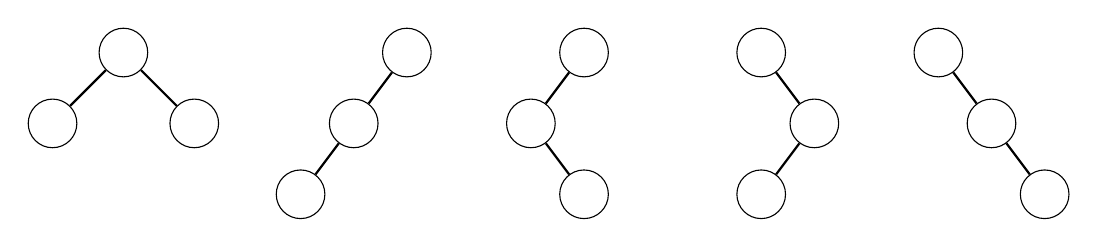
\begin{tikzpicture}[scale=0.9]
\node[draw, circle] (a1) at (0,0) {\phantom{0}};
\node[draw, circle] (a2) at (-1,-1) {\phantom{0}};
\node[draw, circle] (a3) at (1,-1) {\phantom{0}};
\path[draw,thick,-] (a1) -- (a2);
\path[draw,thick,-] (a1) -- (a3);

\node[draw, circle] (b1) at (4,0) {\phantom{0}};
\node[draw, circle] (b2) at (4-0.75,-1) {\phantom{0}};
\node[draw, circle] (b3) at (4-1.5,-2) {\phantom{0}};
\path[draw,thick,-] (b1) -- (b2);
\path[draw,thick,-] (b2) -- (b3);

\node[draw, circle] (c1) at (6.5,0) {\phantom{0}};
\node[draw, circle] (c2) at (6.5-0.75,-1) {\phantom{0}};
\node[draw, circle] (c3) at (6.5-0,-2) {\phantom{0}};
\path[draw,thick,-] (c1) -- (c2);
\path[draw,thick,-] (c2) -- (c3);

\node[draw, circle] (d1) at (9,0) {\phantom{0}};
\node[draw, circle] (d2) at (9+0.75,-1) {\phantom{0}};
\node[draw, circle] (d3) at (9-0,-2) {\phantom{0}};
\path[draw,thick,-] (d1) -- (d2);
\path[draw,thick,-] (d2) -- (d3);

\node[draw, circle] (e1) at (11.5,0) {\phantom{0}};
\node[draw, circle] (e2) at (11.5+0.75,-1) {\phantom{0}};
\node[draw, circle] (e3) at (11.5+1.5,-2) {\phantom{0}};
\path[draw,thick,-] (e1) -- (e2);
\path[draw,thick,-] (e2) -- (e3);
\end{tikzpicture}
\end{center}

Binääripuiden määrä on
\[ C_n = \sum_{i=0}^{n-1} C_{i} C_{n-i-1},\]
missä $i$ on vasemman alipuun koko ja 
$n-i-1$ on oikean alipuun koko.

\section{Inkluusio-ekskluusio}

Inkluusio-ekskluusio
on tekniikka, jonka avulla pystyy laskemaan
joukkojen yhdisteen koon leikkausten
kokojen perusteella ja päinvastoin.
Yksinkertainen esimerkki periaatteesta on kaava
\[ |A \cup B| = |A| + |B| - |A \cap B|,\]
jossa $A$ ja $B$ ovat joukkoja ja $|X|$
tarkoittaa joukon $X$ kokoa.
Seuraava kuva havainnollistaa kaavaa,
kun joukot ovat tason ympyröitä:

\begin{center}
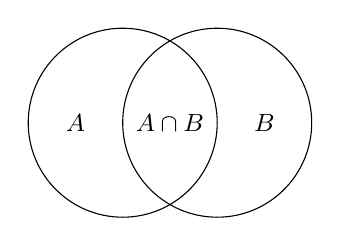
\begin{tikzpicture}[scale=0.8]

\draw (0,0) circle (1.5);
\draw (1.5,0) circle (1.5);

\node at (-0.75,0) {\small $A$};
\node at (2.25,0) {\small $B$};
\node at (0.75,0) {\small $A \cap B$};

\end{tikzpicture}
\end{center}

Tavoitteena on laskea, kuinka suuri on yhdiste $A \cup B$
eli alue, joka on toisen tai kummankin ympyrän sisällä.
Kuvan mukaisesti yhdisteen $A \cup B$ koko
saadaan laskemalla ensin yhteen ympyröiden $A$ ja $B$ koot
ja vähentämällä siitä sitten leikkauksen $A \cap B$ koko.

Samaa ideaa voi soveltaa, kun joukkoja on enemmän.
Kolmen joukon tapauksessa kaavasta tulee
\[ |A \cup B \cup C| = |A| + |B| + |C| - |A \cap B|  - |A \cap C|  - |B \cap C| + |A \cap B \cap C| \]
ja vastaava kuva on

\begin{center}
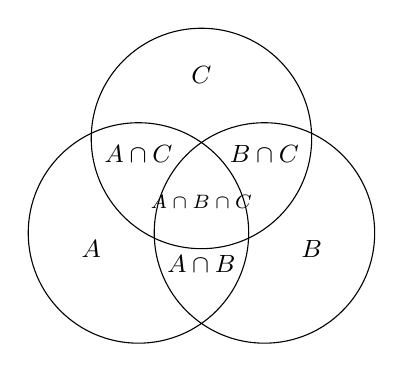
\begin{tikzpicture}[scale=0.8]

\draw (0,0) circle (1.75);
\draw (2,0) circle (1.75);
\draw (1,1.5) circle (1.75);

\node at (-0.75,-0.25) {\small $A$};
\node at (2.75,-0.25) {\small $B$};
\node at (1,2.5) {\small $C$};
\node at (1,-0.5) {\small $A \cap B$};
\node at (0,1.25) {\small $A \cap C$};
\node at (2,1.25) {\small $B \cap C$};
\node at (1,0.5) {\scriptsize $A \cap B \cap C$};

\end{tikzpicture}
\end{center}

Yleisessä tapauksessa yhdisteen $X_1 \cup X_2 \cup \cdots \cup X_n$
koon saa laskettua käymällä läpi kaikki tavat muodostaa
leikkaus joukoista $X_1,X_2,\ldots,X_n$.
Parittoman määrän joukkoja sisältävät leikkaukset
lasketaan mukaan positiivisina ja
parillisen määrän negatiivisina.

Huomaa, että vastaavat kaavat toimivat myös käänteisesti
leikkauksen koon laskemiseen yhdisteiden kokojen perusteella.
Esimerkiksi

\[ |A \cap B| = |A| + |B| - |A \cup B|\]

ja
\[ |A \cap B \cap C| = |A| + |B| + |C| - |A \cup B|  - |A \cup C|  - |B \cup C| + |A \cup B \cup C| .\]

\subsubsection{Esimerkki}

Tarkastellaan esimerkkinä seuraavaa tehtävää:

\begin{task}
Montako tapaa on järjestää permutaatio
$(1,2,\ldots,n)$ uudestaan niin,
että mikään luku ei jää alkuperäiselle paikalleen?
Esimerkiksi jos $n=3$, tapoja on kaksi: $(2,3,1)$ ja $(3,1,2)$
\end{task}

Yksi tapa lähestyä tehtävää on käyttää inkluusio-ekskluusiota.
Olkoon joukko $X_k$ niiden permutaatioiden joukko,
jossa kohdassa $k$ on luku $k$.
Esimerkiksi jos $n=3$, niin joukot ovat seuraavat:
\[
\begin{array}{lcl}
X_1 & = & \{(1,2,3),(1,3,2)\} \\
X_2 & = & \{(1,2,3),(3,2,1)\} \\
X_3 & = & \{(1,2,3),(2,1,3)\} \\
\end{array}
\]
Näitä joukkoja käyttäen ratkaisujen määrä on
\[ n! - |X_1 \cup X_2 \cup \cdots \cup X_n|, \]
eli
riittää laskea joukkojen yhdisteen koko.
Tämä palautuu inkluusio-eks\-kluu\-sion avulla
joukkojen leikkausten kokojen laskemiseen,
mikä onnistuu tehokkaasti.
Esimerkiksi kun $n=3$, joukon $|X_1 \cup X_2 \cup X_3|$ koko on
\[
\begin{array}{lcl}
 & & |X_1| + |X_2| + |X_3| - |X_1 \cap X_2|  - |X_1 \cap X_3|  - |X_2 \cap X_3| + |X_1 \cap X_2 \cap X_3| \\
 & = & 2+2+2-1-1-1+1 \\
 & = & 4, \\
\end{array}
\]
joten ratkaisujen määrä on $3!-4=2$.

Huomaa, että tehtävän voi ratkaista myös toisella
tavalla ilman inkluusio-ekskluusiota
käyttämällä seuraavaa rekursiota:

\begin{equation*}
    f(n) = \begin{cases}
               0               & n = 1\\
               1               & n = 2\\
               (n-1)(f(n-1) + f(n-2)) & n>2 \\
           \end{cases}
\end{equation*}

\section{Burnsiden lemma}

Burnsiden lemma laskee yhdistelmien määrän niin,
että symmetrisistä yhdistelmistä lasketaan
mukaan vain yksi edustaja.
Burnsiden lemman mukaan yhdistelmien määrä on
\[\sum_{k=1}^n \frac{c(k)}{n},\]
missä yhdistelmän asentoa voi muuttaa $n$ tavalla
ja $c(k)$ on niiden yhdistelmien määrä,
jotka pysyvät ennallaan, kun asentoa
muutetaan tavalla $k$.

Tutustumme Burnsiden lemmaan seuraavan tehtävän kautta:

\begin{task}
Helminauhassa on $n$ helmeä,
joista jokaisen väri on väliltä $1,2,\ldots,m$.
Montako erilaista helminauhaa on olemassa?
Kaksi helminauhaa ovat symmetriset,
jos ne voi saada näyttämään samalta pyörittämällä.
\end{task}

\noindent
Esimerkiksi helminauhan
\begin{center}
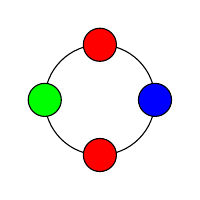
\begin{tikzpicture}[scale=0.7]
\draw[fill=white] (0,0) circle (1);
\draw[fill=red] (0,1) circle (0.3);
\draw[fill=blue] (1,0) circle (0.3);
\draw[fill=red] (0,-1) circle (0.3);
\draw[fill=green] (-1,0) circle (0.3);
\end{tikzpicture}
\end{center}
kanssa symmetriset helminauhat ovat seuraavat:
\begin{center}
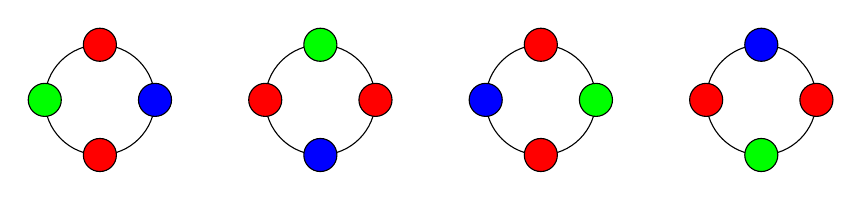
\begin{tikzpicture}[scale=0.7]
\draw[fill=white] (0,0) circle (1);
\draw[fill=red] (0,1) circle (0.3);
\draw[fill=blue] (1,0) circle (0.3);
\draw[fill=red] (0,-1) circle (0.3);
\draw[fill=green] (-1,0) circle (0.3);

\draw[fill=white] (4,0) circle (1);
\draw[fill=green] (4+0,1) circle (0.3);
\draw[fill=red] (4+1,0) circle (0.3);
\draw[fill=blue] (4+0,-1) circle (0.3);
\draw[fill=red] (4+-1,0) circle (0.3);

\draw[fill=white] (8,0) circle (1);
\draw[fill=red] (8+0,1) circle (0.3);
\draw[fill=green] (8+1,0) circle (0.3);
\draw[fill=red] (8+0,-1) circle (0.3);
\draw[fill=blue] (8+-1,0) circle (0.3);

\draw[fill=white] (12,0) circle (1);
\draw[fill=blue] (12+0,1) circle (0.3);
\draw[fill=red] (12+1,0) circle (0.3);
\draw[fill=green] (12+0,-1) circle (0.3);
\draw[fill=red] (12+-1,0) circle (0.3);
\end{tikzpicture}
\end{center}
Tapoja muuttaa asentoa on $n$,
koska helminauhaa voi pyörittää $0,1,\ldots,n-1$
askelta myötäpäivään.
Jos helminauhaa pyörittää 0 askelta,
kaikki $m^n$ väritystä säilyvät ennallaan.
Jos taas helminauhaa pyörittää 1 askeleen,
vain $m$ yksiväristä helminauhaa säilyy ennallaan.

Yleisemmin kun helminauhaa pyörittää $k$ askelta,
ennallaan säilyvien yhdistelmien määrä on
\[m^{\textrm{syt}(k,n)},\]
missä $\textrm{syt}(k,n)$ on lukujen $k$ ja $n$
suurin yhteinen tekijä.
Tämä johtuu siitä, että $\textrm{syt}(k,n)$-kokoiset
pätkät helmiä siirtyvät toistensa paikoille
$k$ askelta eteenpäin.
Niinpä helminauhojen määrä on
Burnsiden lemman mukaan
\[\sum_{i=0}^{n-1} \frac{m^{\textrm{syt}(i,n)}}{n}. \]
Esimerkiksi kun helminauhan pituus on 4
ja värejä on 3, helminauhoja on
\[\frac{3^4+3+3^2+3}{4} = 24. \]

\section{Puiden laskeminen}

Laskemme lopuksi, montako puuta $n$ solmusta
voi muodostaa.
Keskitymme tapaukseen, jossa solmut on numeroitu
ja kaksi puuta ovat erilaiset, jos niiden rakenne
tai numerointi on eri.

Esimerkiksi jos $n=4$, puiden määrä on 16:

\begin{center}
\begin{tikzpicture}[scale=0.9]
\newcommand\puua[6]{
\path[draw,thick,-] (#1,#2) -- (#1-1.25,#2-1.5);
\path[draw,thick,-] (#1,#2) -- (#1,#2-1.5);
\path[draw,thick,-] (#1,#2) -- (#1+1.25,#2-1.5);
\node[draw, circle, fill=white] at (#1,#2) {#3};
\node[draw, circle, fill=white] at (#1-1.25,#2-1.5) {#4};
\node[draw, circle, fill=white] at (#1,#2-1.5) {#5};
\node[draw, circle, fill=white] at (#1+1.25,#2-1.5) {#6};
}
\newcommand\puub[6]{
\path[draw,thick,-] (#1,#2) -- (#1+1,#2);
\path[draw,thick,-] (#1+1,#2) -- (#1+2,#2);
\path[draw,thick,-] (#1+2,#2) -- (#1+3,#2);
\node[draw, circle, fill=white] at (#1,#2) {#3};
\node[draw, circle, fill=white] at (#1+1,#2) {#4};
\node[draw, circle, fill=white] at (#1+2,#2) {#5};
\node[draw, circle, fill=white] at (#1+3,#2) {#6};
}

\puua{0}{0}{1}{2}{3}{4}
\puua{4}{0}{2}{1}{3}{4}
\puua{8}{0}{3}{1}{2}{4}
\puua{12}{0}{4}{1}{2}{3}

\puub{0}{-3}{1}{2}{3}{4}
\puub{4.5}{-3}{1}{2}{4}{3}
\puub{9}{-3}{1}{3}{2}{4}
\puub{0}{-4.5}{1}{3}{4}{2}
\puub{4.5}{-4.5}{1}{4}{2}{3}
\puub{9}{-4.5}{1}{4}{3}{2}
\puub{0}{-6}{2}{1}{3}{4}
\puub{4.5}{-6}{2}{1}{4}{3}
\puub{9}{-6}{2}{3}{1}{4}
\puub{0}{-7.5}{2}{4}{1}{3}
\puub{4.5}{-7.5}{3}{1}{2}{4}
\puub{9}{-7.5}{3}{2}{1}{4}
\end{tikzpicture}
\end{center}

Osoittautuu, että $n$ solmusta voi muodostaa $n^{n-2}$
numeroitua puuta.
Tämä tulos tunnetaan nimellä Cayleyn kaava.

\subsubsection{Prüfer-koodi}

Prüfer-koodi on $n-2$ luvun jono,
joka kuvaa puun rakenteen.
Koodi muodostuu poistamalla puusta
joka askeleella lehden, jonka numero on pienin,
ja lisäämällä lehden vieressä olevan solmun
tunnus koodiin.

Esimerkiksi puun

\begin{center}
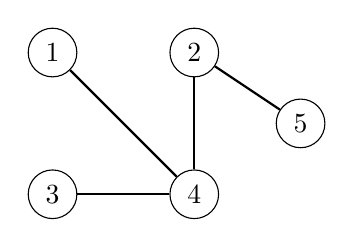
\begin{tikzpicture}[scale=0.9]
\node[draw, circle] (1) at (2,3) {$1$};
\node[draw, circle] (2) at (4,3) {$2$};
\node[draw, circle] (3) at (2,1) {$3$};
\node[draw, circle] (4) at (4,1) {$4$};
\node[draw, circle] (5) at (5.5,2) {$5$};

%\path[draw,thick,-] (1) -- (2);
%\path[draw,thick,-] (1) -- (3);
\path[draw,thick,-] (1) -- (4);
\path[draw,thick,-] (3) -- (4);
\path[draw,thick,-] (2) -- (4);
\path[draw,thick,-] (2) -- (5);
%\path[draw,thick,-] (4) -- (5);
\end{tikzpicture}
\end{center}
Prüfer-koodi on $(4,4,2)$,
koska ensin poistetaan solmu 1,
sitten solmu 3 ja lopuksi solmu 5.

Jokaiselle puulle voidaan laskea
Prüfer-koodi, minkä lisäksi
Prüfer-koodista pystyy palauttamaan
yksikäsitteisesti puun rakenteen.
Niinpä erilaisia puita on yhtä monta
kuin Prüfer-koodeja eli $n^{n-2}$.


% \subsubsection*{Yhdistelmät}
% 
% Jos yhdistelmä muodostuu $n$ osasta ja jokainen osa
% voidaan valita $k$ tavalla, yhdistelmiä on yhteensä $k^n$.
% Esimerkiksi $n$-pituisia bittijonoja on $2^n$,
% koska jokainen jonon bitti voidaan valita 2 tavalla.
% 
% Yleisemmin jos yhdistelmä muodostuu $n$ osasta,
% joista osan 1 voi valita $k_1$ tavalla,
% osan 2 voi valita $k_2$ tavalla, jne.,
% yhdistelmien määrä on $k_1 \cdot k_2 \cdots k_n$.
% 
% \subsubsection*{Permutaatiot}
% 
% Permutaatio tarkoittaa joukon alkioiden järjestystä.
% Jos joukossa on $n$ alkiota,
% niin siitä voi muodostaa $n!$ permutaatiota,
% koska ensimmäinen alkio voidaan valita $n$ tavalla,
% toinen $(n-1)$ tavalla, jne.
% Esimerkiksi kirjaimet \texttt{ABC} voidaan järjestää
% 6 tavalla:
% \texttt{ABC}, \texttt{ACB}, \texttt{BAC}, \texttt{BCA},
% \texttt{CAB} ja \texttt{CBA}.
% 
% \subsubsection*{Rekursiokaava}
% 
% Kombinatorisen tehtävän ratkaisun pystyy usein ilmaisemaan
% rekursiolla, jolloin vastauksen saa laskettua tehokkaasti
% dynaamisella ohjelmoinnilla.
% Näin on esimerkiksi seuraavassa tehtävässä:
% 
% \begin{task}
% Tehtäväsi on laskea, monessako $n$ bitin jonossa
% ei ole vierekkäin kahta ykkösbittiä.
% Esimerkiksi jos $n=4$, vastaus on 8,
% koska bittijonot ovat \texttt{0000}, \texttt{0001},
% \texttt{0010}, \texttt{0100}, \texttt{0101},
% \texttt{1000}, \texttt{1001} ja \texttt{1010}.
% \end{task}
% 
% Vastaus selviää funktiolla $f(n,k)$,
% jossa $n$ on bittijonon pituus ja $k$ on viimeinen bitti (0 tai 1).
% Tätä funktiota käyttäen $n$ bitin jonojen määrä
% on summa $f(n,0)+f(n,1)$.
% Rekursiivinen kaava on seuraava:
% 
% \begin{equation*}
%     f(n,k) = \begin{cases}
%                1               & n = 1\\
%                f(n-1,0)+f(n-1,1) & k = 0\\
%                f(n-1,0) & k = 1\\
%            \end{cases}
% \end{equation*}
% 
% Kaavan ideana on, että jos viimeinen bitti on 0,
% sitä ennen voi olla sekä bitti 0 että bitti 1,
% ja jos viimeinen bitti on 1, sitä ennen on
% pakko olla bitti 0.
% 
% 
% \section{Binomikerroin}
% 
% \subsubsection*{Hatut ja pallot}
% 
% Binomikertoimen avulla voi ratkaista myös seuraavan tehtävän:
% 
% \begin{task}
% Rivissä on $n$ hattua, joihin sijoitetaan $m$ palloa.
% Montako erilaista tapaa tähän on?
% Esimerkiksi jos $n=3$ ja $m=2$, niin tapoja on 6:
% $[0,0,2]$, $[0,1,1]$, $[0,2,0]$, $[1,0,1]$, $[1,1,0]$,
% $[2,0,0]$.
% \end{task}
% 
% \noindent
% Ratkaisu tehtävään on ${n+m-1 \choose m}$.
% Jokaisen sijoitustavan voi ilmaista merkkijonona, jossa \texttt{o}
% kuvaa palloa ja \texttt{|} on kahden hatun raja.
% Merkkijonon pituus on $n+m-1$, koska palloja on $m$
% ja hatun rajoja on $n-1$,
% ja siitä valitaan $m$ paikkaa palloille.
% Esimerkiksi sijoitustapaa $[1,0,1]$
% vastaa merkkijono \texttt{o||o}.
% 
% 
